%%%%%%%%%%%%%%%%%%%%%%%%%%%%%%%%%%%%%%%%%%%%%%%%%%%%%%%%%%%%%%%%%%%%%%%%%%%%%%%
\documentclass[a4paper,12pt]{article}

%%%%%%%%%%%%%%%%%%%%%%%%%%%%%%%%%%%%%%%%%%%%%%%%%%%%%%%%%%%%%%%%%%%%%%%%%%%%%%%

\usepackage{extsizes}
\usepackage{cmap}
\usepackage[T2A]{fontenc}
\usepackage[utf8x]{inputenc}
\usepackage[english, russian]{babel}
\usepackage{misccorr}
\usepackage{amssymb,amsfonts,amsmath,amsthm}  % математические дополнения от АМС
\usepackage{envmath}  % многострочные формулы EqSystem
\usepackage{indentfirst} % Включение отступа первой строки раздела
\usepackage[usenames,dvipsnames]{color} % названия цветов

%%%%%%%%%%%%%%%%%%%%%%%%%%%%%%%%%%%%%%%%%%%%%%%%%%%%%%%%%%%%%%%%%%%%%%%%%%%%%%%

	% выбрать цвета:
% \definecolor{BlueGreen}{RGB}{49,152,255}

%%%%%%%%%%%%%%%%%%%%%%%%%%%%%%%%%%%%%%%%%%%%%%%%%%%%%%%%%%%%%%%%%%%%%%%%%%%%%%%

	% назначить цвета при подключении hyperref
\usepackage[unicode, colorlinks, urlcolor=magenta, linkcolor=black, pagecolor=black]{hyperref}
	% linkcolor=
	% цвет гиперссылок внутри документа, по-умолчанию red
	% pagecolor=
	% цвет гиперссылок на другие страницы внутри документа, по-умолчанию red
	% filecolor=
	% цвет гиперссылок, открывающих локальные файлы, по-умолчанию cyan
	% anchorcolor=
	% цвет текста мишени, по-умолчанию black
	% citecolor=
	% цвет библиографических ссылок, по-умолчанию green
	% urlcolor=
	% цвет гиперссылок на сетевые ресурсы, по-умолчанию magenta

%%%%%%%%%%%%%%%%%%%%%%%%%%%%%%%%%%%%%%%%%%%%%%%%%%%%%%%%%%%%%%%%%%%%%%%%%%%%%%%

	% улучшенное форматирование таблиц
\usepackage{makecell} 
\usepackage{multirow} 

%%%%%%%%%%%%%%%%%%%%%%%%%%%%%%%%%%%%%%%%%%%%%%%%%%%%%%%%%%%%%%%%%%%%%%%%%%%%%%%

	% подчеркивания
\usepackage{ulem}

%%%%%%%%%%%%%%%%%%%%%%%%%%%%%%%%%%%%%%%%%%%%%%%%%%%%%%%%%%%%%%%%%%%%%%%%%%%%%%%

	% для вставки изображений
\usepackage{graphicx} 
	%где искать изображения
\graphicspath{{img/}}

%%%%%%%%%%%%%%%%%%%%%%%%%%%%%%%%%%%%%%%%%%%%%%%%%%%%%%%%%%%%%%%%%%%%%%%%%%%%%%%
	
	% поля страницы 
\usepackage{geometry}
\geometry{left=3cm,right=2cm,top=3cm,bottom=3cm,bindingoffset=0cm}

%%%%%%%%%%%%%%%%%%%%%%%%%%%%%%%%%%%%%%%%%%%%%%%%%%%%%%%%%%%%%%%%%%%%%%%%%%%%%%%

	% Cтиль оформления chapter
% \usepackage[Glenn]{fncychap} 
	% Всего имеется семь возможных стилей: 
	% Sonny, Lenny, Glenn, Conny, Rejne, Bjarne, Bjornstrup.

%%%%%%%%%%%%%%%%%%%%%%%%%%%%%%%%%%%%%%%%%%%%%%%%%%%%%%%%%%%%%%%%%%%%%%%%%%%%%%%

	%Колинтулы страниц
\usepackage{fancyhdr} 

%%%%%%%%%%%%%%%%%%%%%%%%%%%%%%%%%%%%%%%%%%%%%%%%%%%%%%%%%%%%%%%%%%%%%%%%%%%%%%%

	% полуторный интервал
\linespread{1.3} 

	% стиль пробелов: французский - все пробелы примерно одинаковые
\frenchspacing 

	% Элементы списка второго уровня с скобочкой вместо точки
\renewcommand{\labelenumii}{\theenumii)} 

%%%%%%%%%%%%%%%%%%%%%%%%%%%%%%%%%%%%%%%%%%%%%%%%%%%%%%%%%%%%%%%%%%%%%%%%%%%%%%%  % преамбула
%%%%%%%%%%%%%%%%%%%%%%%%%%%%%%%%%%%%%%%%%%%%%%%%%%%%%%%%%%%%%%%%%%%%%%%%%%%%%%%

\newcommand{\labauthor}{Сарафанов Ф.\,Г.}
\newcommand{\labauthors}{Сарафанов Ф.\,Г.}
% \newcommand{\labauthors}{Сарафанов Ф.\,Г., Сидоров Д.\,А.}
\newcommand{\labnumber}{17}
\newcommand{\labtheme}{Осциллограф}


\newcommand{\ddt}{$\ \pm\ 0.2\ \text{с}$}
\newcommand{\ddtv}{$\ \pm\ 0.8\ \text{с}$}
\newcommand{\ddh}{$\ \pm\ 0.1\ \text{см}$}
\newcommand{\dm}{\Delta{}m}
\newcommand{\Dh}{\Delta{}x}
\newcommand{\Dl}{\Delta{}(\lambda)}
\newcommand{\dmsr}{<\Delta{}m>}
\newcommand{\el}{\varepsilon(\lambda)}

\usetikzlibrary{%
    decorations.pathreplacing,%
    decorations.pathmorphing,%
    arrows,%
    patterns
}
\newcommand{\Scale}{1}
\newcommand{\lft}{9}
\newcommand{\rft}{10.43*1.5}
\newcommand{\Xstep}{1.5}
\newcommand{\Ystep}{1.5*20}
\newcommand{\Radius}{0.1}
\newcommand{\Color}{black}


%%%%%%%%%%%%%%%%%%%%%%%%%%%%%%%%%%%%%%%%%%%%%%%%%%%%%%%%%%%%%%%%%%%%%%%%%%%%%%%
%%%%%%%%%%%%%%%%%%%%%%%%%%%%%%%%%%%%%%%%%%%%%%%%%%%%%%%%%%%%%%%%%%%%%%%%%%%%%%%
	%применим колонтитул к стилю страницы
\pagestyle{fancy} 
	%очистим "шапку" страницы
\fancyhead{} 
	%слева сверху на четных и справа на нечетных
\fancyhead[LE,RO]{\labauthors} 
	%справа сверху на четных и слева на нечетных
\fancyhead[LO, RE]{Отчёт по лабораторной работе №\labnumber} 
	%очистим "подвал" страницы
\fancyfoot{} 
	% номер страницы в нижнем колинтуле в центре
\fancyfoot[CO,CE]{\thepage} 

%%%%%%%%%%%%%%%%%%%%%%%%%%%%%%%%%%%%%%%%%%%%%%%%%%%%%%%%%%%%%%%%%%%%%%%%%%%%%%% % колинтулы на страницах
%%%%%%%%%%%%%%%%%%%%%%%%%%%%%%%%%%%%%%%%%%%%%%%%%%%%%%%%%%%%%%%%%%%%%%%%%%%%%%%

\begin{document}

\begin{titlepage}

\begin{center}

{\small\textsc{Нижегородский государственный университет имени Н.\,И. Лобачевского}}
\vskip 1pt \hrule \vskip 3pt
{\small\textsc{Радиофизический факультет}}

\vfill

{\Large Отчет по лабораторной работе №\labnumber\vskip 12pt\bfseries \labtheme}
	
\end{center}

\vfill
	
\begin{flushright}
	{Выполнил студент 410 группы\\ \labauthor\vskip 12pt Принял:\\ Менсов С.\,Н.}
\end{flushright}
	
\vfill
	
\begin{center}
	Нижний Новгород, 2016
\end{center}

\end{titlepage}



\tableofcontents

\newpage
\section{Описание лабораторной установки}

\textbf{Цель работы:} ознакомление с устройством электронного осциллографа; изучение принципов работы развертки, усилителей вертикального и горизонтального каналов, получение фигур Лиссажу, изучение частотных свойств вертикального усилителя.
\vspace{1.5em}

\textbf{Оборудование:}
Осциллограф С1-1 (ЭО-7), генератор низкочастотных сигналов ГЗ-109
\vspace{1.5em}

\textbf{Приборные погрешности:} Класс точности вольтметра - 2.5, погрешности генератора: $\Delta{\nu}=2+\frac{50}{\nu}$ (20--200 Гц), $\Delta{\nu}=1+\frac{50}{\nu}$ (200 Гц--200 кГц).
\vspace{1.5em}

Электронный осциллограф — прибор, предназначенный в основном для исследования быстропротекающих процессов в электрических цепях (или не электрических процессов с помощью соответствующих преобразователей представленных в виде электрических сигналов).

В работе использован осциллограф C1-1 (ЭО-7). Его упрощенная блок-схема приведена на рисунке (рис. \ref{fig:cxem})

\begin{figure}[ht!]
	\centering
	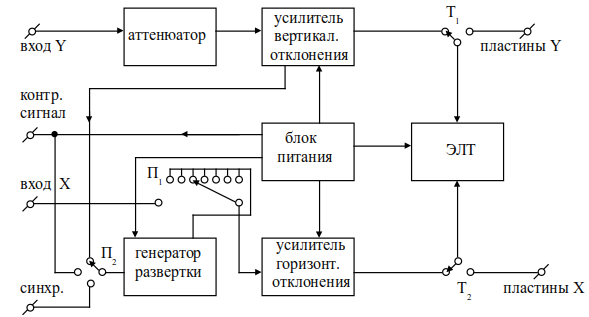
\includegraphics[width=0.8\textwidth]{chem.png}
	\caption{Упрощенная блок-схема осциллографа}
	\label{fig:chem}
\end{figure}

\begin{figure}[ht!]
	\centering
	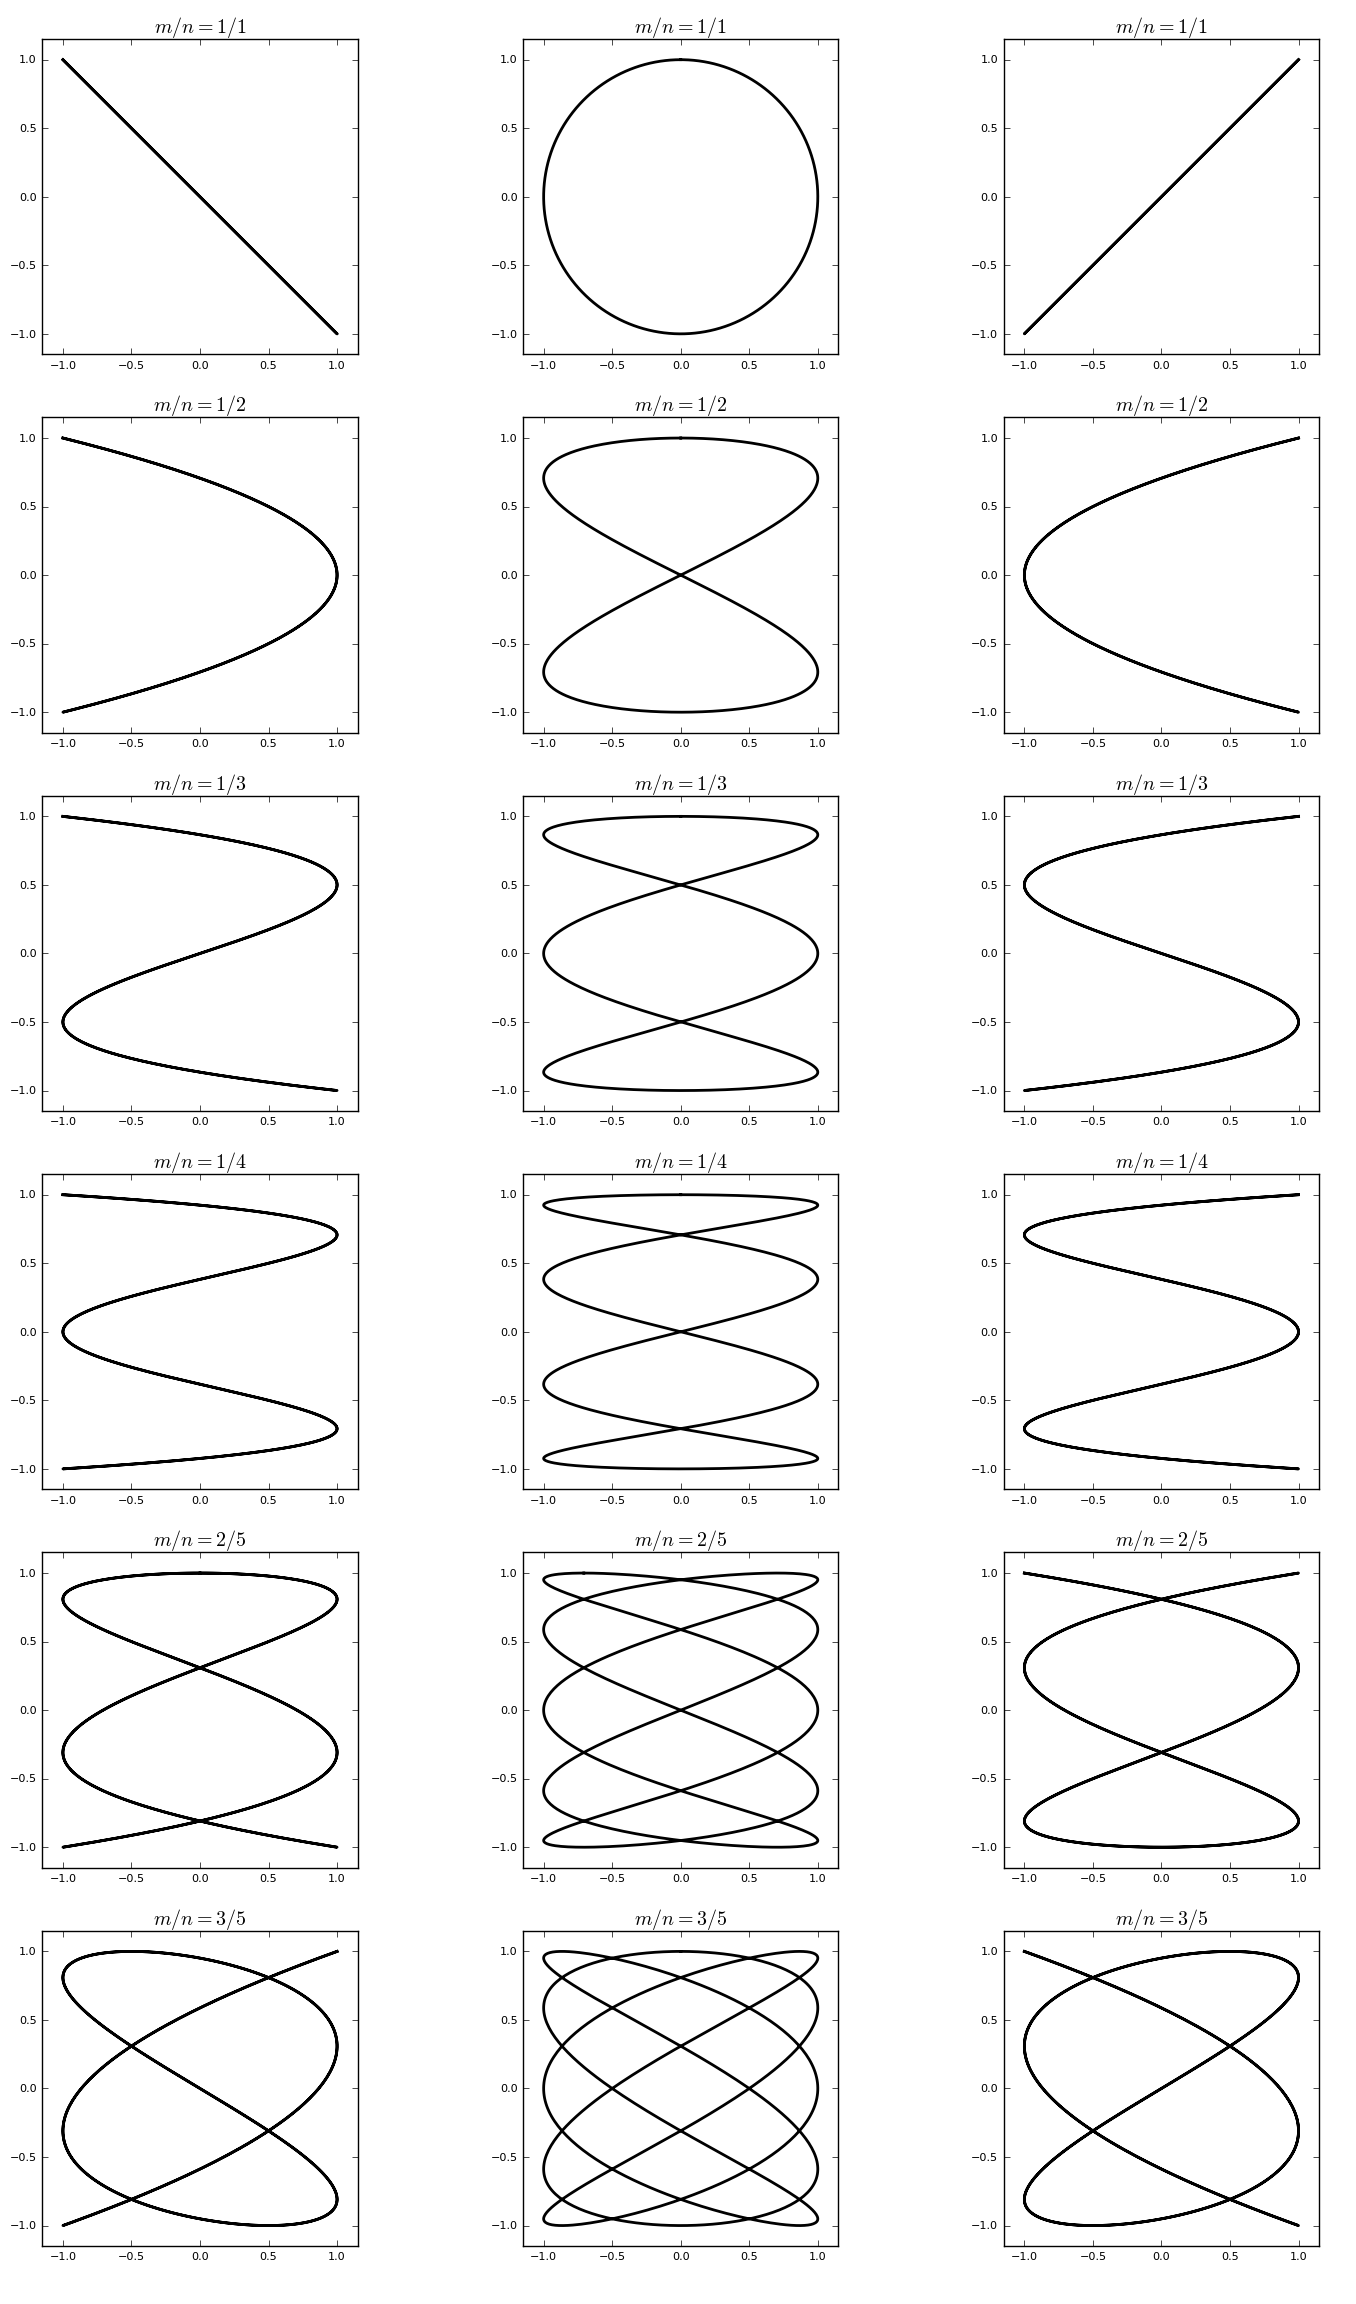
\includegraphics[width=0.8\textwidth]{lissajous3.png}
	\caption{Фигуры Лиссажу для $\frac{m}{n}=1;2;3;4;\frac{5}{2};\frac{5}{3}$}
	\label{fig:cxem}
\end{figure}



На отклоняющие пластины подается (не одновременно во время опытов) переменное напряжение $U_\text{в}$ ($U_\text{г}$) с эффективным значением $75$ вольт и частотой $50$ Гц. 

Вокруг трубки намотан соленоид с диаметром 7 см, плотность намотки 



\section{Измерение удельного заряда электрона методом отклонения земным магнитным полем}

В лабораторной работе исследуется .

Погрешности, используемые в работе: 

Запишем :
\begin{EqSystem}
\end{EqSystem}

Спроецируем на ось X, направленную :
\begin{EqSystem}
	\label{eq:}
\end{EqSystem}

\subsection{Вывод}

В результате проделанной работы были выполнены следующие пункты.

Опровергнута гипотеза 

Снята линейная зависимость  откуда сделан вывод о .

Снята зависимость ,
для которой расчитана соответствующая погрешность (\ref{})

Оценены коэффициенты $\lambda$  и $F_0$ методом .

Изучено уравнение динамики вращательного движения (ОУДВД) и физический смысл момента инерции, а также методы его вычисления.

Рассчитано значение коэффициента 

Определена правильность определения

Сравнение , полученного разными способами, показывает: в пределах погрешностей измерений можно утверждать следующее: 


В пределах погрешностей измерений были построены графики зависимостей.

В работе рассчитаны погрешности для всех косвенных измерений, размеры прямоугольников ошибок. 

Все точки на графиках укладываются на  теоретические графики в пределах размеров их прямоугольников ошибок.

Подтверждена 

\begin{figure}[h!]
	\centering
	% \includegraphics[]{}	
	\begin{tikzpicture}
	\hspace{-1cm}
		\draw[fill,yellow!60] 	
	% (1.5,0) --
	(0,0) --
	(3.0000,1.0000) --
	(4.5000,2.0000) --
	(6.0000,3.0000) --
	(6.7500,4.0000) --
	(7.5000,5.0000) --
	(9.0000,6.0000) --
	(9.7500,7.0000) --
	(10.5000,8.0000) --
	(12,\lft) --
	(\rft,\lft) --
	(\rft,-\lft) --
	(15.0000,-8.0000) --
	(13.5000,-7.0000) --
	(10.5000,-6.0000) --
	(9.0000,-5.0000) --
	(6.7500,-4.0000) --
	(5.2500,-3.0000) --
	(3.7500,-2.0000) --
	(2.2500,-1.0000) -- cycle;
			

\draw[step=.1cm , gray!20] (0,-\lft) grid (\rft ,\lft);
\draw[step=0.5cm , gray!50] (0,-\lft) grid (\rft ,\lft);
\draw[step=1cm , gray!80] (0,-\lft) grid (\rft ,\lft);


\draw[-{>[scale=1.0]}] (-0,0) -- (10*1.5 +1 ,0) node[anchor=north west] {\scalebox{1.5}{$A$}};
\draw[->] (0,-\lft) -- (0,\lft+1 ) node[anchor=east] {\scalebox{1.5}{$\frac{\nu_\text{с}-\nu_\text{р}}{\nu_\text{р}}$}};


\foreach \x in {1,2,3,4,5,6,7,8,9,10} {
	\draw (\x*\Xstep,0.05) -- (\x*\Xstep,-0.05);
	\draw (\x*\Xstep,0) node[anchor=north] {\scalebox{1.5}{$\x$}};
}

\foreach \y in {-0.3,-0.2,-0.1, 0, 0.1,0.2,0.3} {
	\draw (0.05,\y*\Ystep) -- (-0.05,\y*\Ystep);
	\draw (0,\y*\Ystep) node[anchor=east] {\scalebox{1.5}{$\y$}};
}

% \draw[blue] (15,0.5) node[anchor=east] {\scalebox{1.4}{Синхронизованная зона}};
% \draw[blue] (9.5,8.2) node[anchor=east] {\scalebox{1.4}{Несинхронизованная зона}};
% \draw[blue] (9.5,-8.3) node[anchor=east] {\scalebox{1.4}{Несинхронизованная зона}};
\input{experience/table.out}		
	\end{tikzpicture}
	\caption{Caption here}
	\label{fig:figure1}
\end{figure}

% \newpage
% \section*{Приложение 1. Графики зависимостей} % (fold)
% \label{sec:figures}

% section figures (end)

\end{document}
